\subsubsubsection{Ažuriranje ponude snabdevača}

\begin{itemize}
    \item Kratak opis:
        \begin{itemize}
            \item Registrovani snabdevač ažurira svoju ponudu.
        \end{itemize}
    \item Učesnici:
        \begin{itemize}
            \item Snabdevač
        \end{itemize}
    \item Preduslovi:
        \begin{itemize}
            \item Snabdevač mora biti registrovan i ulogovan na aplikaciju.
        \end{itemize}
    \item Postuslovi:
        \begin{itemize}
            \item Podaci su uspešno sačuvani u bazi podataka.
        \end{itemize}
    \item Osnovni tok:
        \begin{enumerate}
            \item Snabdevač bira opciju da ažurira svoju ponudu.
            \item Sistem prikazuje snabdevaču formu za izmenu ponude.
            \item Snabdevač ažurira dostupne namernice i njihovu količinu i potvrđuje izmene.
            \item Sistem čuva izmene u bazi podataka.
            \item Sistem prikazuje poruku o uspešnosti. 
        \end{enumerate}
\end{itemize}


\begin{figure}[H]
\begin{center}
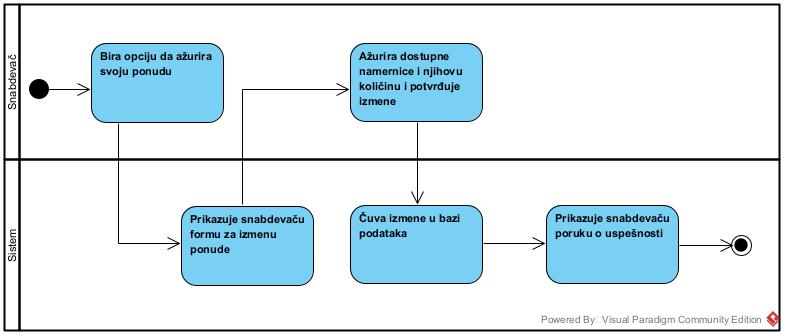
\includegraphics[width=\textwidth]{Pictures/activity_update_supplier_account.jpg}
\end{center}
    \caption{Dijagram aktivnosti ažuriranja ponude snabdevača}
\label{fig:ActivityUpdateSupplierAccount}
\end{figure}
